\documentclass{article}
\usepackage{graphicx}
\usepackage{float}
\usepackage{amsmath}
\usepackage{enumerate}
\usepackage{amsfonts}

\setlength{\parindent}{0pt}

\begin{document}

\title{Lecture 1.1: An Introduction to Limits}
\author{Professor Leonard}
\maketitle

\section{Limits}

Limits are the basis of calculus. There are two goals in calculus:

\begin{enumerate}
    \item Given any curve, find the slope of a curve at a point (find the tangent to a
        curve at a point).
    \item Given any curve defined by a function, can you between two points find the area
        under the curve?
\end{enumerate}

\subsection{Tangent Problem}

If you give me an arbitrary curve, and give me a point $p$, I need to find the slope of
the curve at point $p$. If we have the slope and we have the point, we can make the
tangent line. \\

\emph{Tangent line.} A tangent line is a line that touches at exactly one point and is
"parallel to the curve at that point.\\

One problem if we only have one point and no slope is we can't draw a line---we need at
least one more point. We can find another point along the curve and connect the two to
form a secant line.\\

\emph{Secant line.} A secant line is a line that intersects a curve at two points (see
Figure \ref{fig:secant}).\\

\begin{figure}[H]
    \centering
    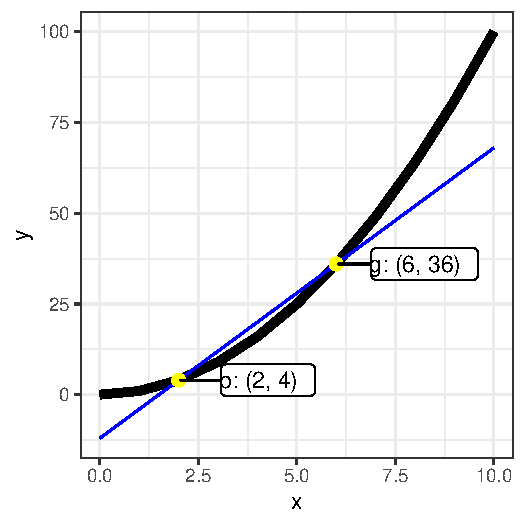
\includegraphics{secant.pdf}
    \caption{A secant line intersects two points on a curve.}
    \label{fig:secant}
\end{figure}

So in Figure \ref{fig:secant}, how could we come up with a secant line that's a better
approximation of the tangent line? We can incrementally move $g$ closer and closer to $p$
and observe that it becomes a better approximation.

\begin{figure}[H]
    \centering
    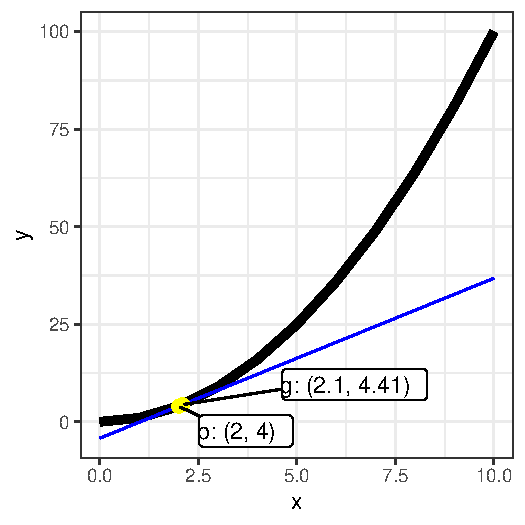
\includegraphics{updated_secant.pdf}
    \caption{Moving points closer together results in a more accurate estimation of the
    tangent line}
    \label{fig:updated_secant}
\end{figure}

As points $p$ and $g$ come closer together in Figure \ref{fig:updated_secant}, we see the
line is a better approximation of the tangent line.\\

\emph{Note:} $p$ can't equal $q$ because two points are needed to make a line.\\

\textbf{Big idea for limits.} How close can two points get to each other without being the
same point? The solution is to let two points get infinitesimally close together without actually
equalling each other. If this is the case, then the secant will be identical to the
tangent. So a limit is letting something get infinitesimally close without touching it.

\subsubsection{Example of finding tangent line}

For function $f(x) = x^2$, can we find the tangent line at $(1, 1)$? 

\begin{enumerate}
    \item We can think of a general second point of the form $q: (x, x^2)$
    \item Recall point slope formula: $y - y_1 = m(x - x_1)$
    \item For a tangent line, the formula is similar but we'd substitute in the slope of
        the tangent line: $y - y_1 = M_{tan}(x - x_1)$
    \item Substitute in the fixed point $(1, 1)$. 
    \item Make the line into a secant, and move $q$ closer to $(1, 1)$ to find the
        tangent.
    \item Derive a general slope for $M_{sec} = \frac{x^2 - 1}{x - 1}$. This holds because
        we know the general form of $q: (x, x^2)$.
    \item As $Q \rightarrow P$, then $M_{sec} \rightarrow M_{tan}$.
    \item But notice that, in the general slope formula for $M_{sec}$, moving $q$ all the
        way to $p$ results in $0/0$, which doesn't work. 
    \item But also notice that the general slope formula for $M_{sec}$ can be simplified:

        \begin{align*}
            M_{sec} &= \frac{x^2 - 1}{x-1}\\
            &= \frac{(x+1)(x-1)}{x-1}\\
            &= x + 1
        \end{align*}

    \item Remember, after a simplification, you don't get rid of domain restrictions. So,
        as $q \rightarrow p$, $M_{sec} = x + 1 \rightarrow 2$.
    \item But you are allowed to make a jump to make a claim that $M_{tan} = 2$. And
        solving for slope intercept form gives you the equation of a tangent line at point
        $(1, 1)$, which is $y = 2x - 1$.


\end{enumerate}

\begin{figure}[H]
    \centering
    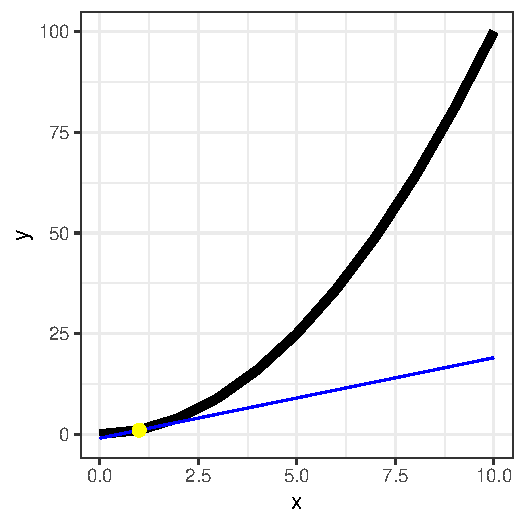
\includegraphics{tangent.pdf}
    \caption{A tangent line at point $p: (1, 1)$}
    \label{fig:tangent}
\end{figure}

\subsection{The area problem}

The other big calculus idea is finding the area under a curve. The basic idea is that
you're drawing many many tiny rectangles in that space under the curve, then taking the
area of the rectangles. As the number of rectangles approaches infinity, the approximation
of area under the curve approaches perfection.

\subsection{Back to limits}

A \emph{limit} tells you what a function does as the variable approaches a specific
value.\\

\emph{Example.} For $f(x) = x^2$, what happens as $x \rightarrow 2$?\\

The way he's working through this is to put a table on the board mapping $x$ to $x^2$ for
values approaching $2$ on both the high and low ends. The function has to approach the
same value from both the left and the right for the limit to exist. Write a limit like:
$\lim_{x\to 2} x^2 = 4$. We actually don't care about what happens when $x$ \emph{gets} to
that number.

$$
\lim_{x\to a} f(x) = L
$$

To talk about a limit coming from the right hand side: $\lim_{x\to a^+} f(x) = L$. Add
negative sign for from the left. These quantities can be pretty different depending if
there's a big discontinuity in the function around the limit. \\

\emph{Note:} In order from a limit to exist at a point, you must have $\lim_{x \to a^-}
f(x) = \lim_{x \to a^+} f(x).$ This suggests that if you have a limit around a big
discontinuity, that there is no limit "at a point". Ah, so this plus / minus notation is
specific to finding the limit coming from a certain side. Without the sign, it's like the
general limit and, if it converges at a point, it'll have a single solution. 

\begin{figure}[H]
    \centering
    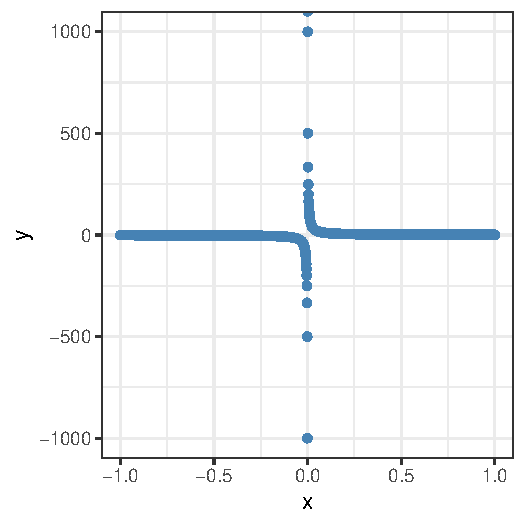
\includegraphics{zero_limit.pdf}
    \caption{$\lim_{x \to 0}f(x)$}
    \label{fig:zero-limit}
\end{figure}


The limit is $\infty$ !!!\\

So actually, because the function goes to pos or neg infinity as it approaches from either
side, it doesn't converge on a single limit, and so we'd say the limit doesn't exist.\\

He's talking a bit about the general case of thinking about an infinity limit as you
approach some x: $\lim_{x\to a^+} f(x) = \infty$, $\lim_{x \to a^+} = f(x) -\infty$,
$\lim_{x\to a^-} f(x) \infty$, $\lim_{x\to a^-} f(x) - \infty$. Should be able to
understand what happens to the function at all four of these cases.

\end{document}




